\documentclass[11pt]{article}
\usepackage[a4paper,margin=1in]{geometry}
\usepackage{amsmath,amssymb,amsfonts,mathtools}
\usepackage{graphicx}
\usepackage{booktabs}
\usepackage{enumitem}
\usepackage{lineno}
\usepackage[hidelinks]{hyperref}
\usepackage{authblk}
\setlength{\parskip}{0.3em}
\newcommand{\Om}{\Omega}
\newcommand{\eps}{\varepsilon}
\newcommand{\half}{\tfrac12}

\title{\textbf{Coupled dispersion characteristics of a two-flexible-plate
structural--acoustic waveguide with low-Mach Poiseuille flow:\\
an asymptotic analysis}}
\author[1]{Ashray Saxena}
\affil[1]{\small Department of Mechanical Engineering, Birla Institute of Technology \& Science Pilani, Pilani Campus, India}
\date{\today}

\begin{document}
\maketitle

\begin{abstract}
\noindent
Analytical expressions are derived, using asymptotics, for the fluid--structure coupled wavenumbers
of a two-dimensional structural--acoustic waveguide in which a fluid column is bounded by \emph{two
flexible plates}. This generalises the single-flexible-plate/rigid-wall waveguide of Sarkar \& Sonti
[\emph{J.\ Sound Vib.}\ \textbf{306} (2007) 657] and the symmetric-mode model of Fahy. The coupled
dispersion relation is obtained in closed form and shown to factorise, for identical plates, into
decoupled \emph{symmetric} and \emph{antisymmetric} families; the rigid-wall limit recovers the
Sarkar--Sonti relation exactly. A complete first-order asymptotic catalogue in the fluid-loading
parameter~$\eps$ is constructed for both families --- structural, plane-wave and cut-on branches,
together with the local $\sqrt{\eps}$ expansions that resolve the avoided crossings at coincidence and
at each cut-on --- and every expression is validated against exact numerical roots. The single
rigid-duct cut-on ladder is shown to split into interleaved even (symmetric) and odd (antisymmetric)
ladders that swap parity as $\eps$ increases (rigid$\to$pressure-release migration). A uniform
Poiseuille mean flow is then introduced; the perturbation field obeys the Pridmore--Brown equation
with plate-admittance boundary conditions, and a closed-form $O(M)$ correction to every coupled
wavenumber is derived by a Fredholm solvability condition and extended to $O(M^2)$ with an explicit
convection/shear decomposition. A critical layer is shown to appear when the axial phase Mach number
reaches unity, at $M_{\rm crit}=\Om/\xi\approx\sqrt{\Om}$, i.e.\ only for the subsonic structural wave
below coincidence; its inviscid (Frobenius) structure, causal continuation, and viscous regularisation
(thickness $\sim Re^{-1/3}$, phase jump $-\mathrm{i}\pi$) are analysed. A viscous linearised
Navier--Stokes solution shows the eigenvalue is regular above $M_{\rm crit}$ and that the discrete
wall modes are \emph{not} absorbed by the interior critical layer --- their decay is
wall-Stokes-dominated ($\propto Re^{-1/2}$) and vanishes inviscidly. The results are confirmed by
three mutually independent methods --- Runge--Kutta shooting, Chebyshev spectral collocation, and a
primitive-variable linearised-Euler formulation reduced symbolically to Pridmore--Brown form ---
which agree to $\sim\!10^{-9}$.
\\[1ex]
\noindent\textbf{Keywords:} structural acoustics; fluid--structure coupling; dispersion relation;
asymptotic analysis; Pridmore--Brown equation; critical layer.
\end{abstract}

\section*{Nomenclature}
\noindent\begin{tabular}{@{}ll@{}}
$a$ & fluid-column height (plate separation)\\
$c,\ \rho$ & sound speed, fluid density\\
$D_j=E_jI_j$ & flexural rigidity of plate $j$ ($I_j=h_j^3/[12(1-\nu_j^2)]$)\\
$E_j,\ \nu_j,\ h_j,\ \rho_{p,j}$ & Young's modulus, Poisson ratio, thickness, density of plate $j$\\
$G_j=D_jk_x^4-m_j\omega^2$ & in-vacuo plate (bending) operator\\
$f(\eta)=4\eta(1-\eta)$ & normalised Poiseuille velocity profile\\
$k=\omega/c$ & acoustic wavenumber\\
$k_x,\ k_y=\sqrt{k^2-k_x^2}$ & axial and transverse wavenumbers\\
$k_c,\ \omega_c$ & coincidence wavenumber and frequency of plate~1\\
$l=k_ca$ & non-dimensional gap\\
$m_j=\rho_{p,j}h_j$ & mass per unit area of plate $j$\\
$M=U_0/c$ & centreline Mach number\\
$p,\ \hat p=p/\rho c^2$ & acoustic pressure perturbation (dimensional, non-dimensional)\\
$Re=ca/\nu$ & acoustic Reynolds number ($\nu$ = kinematic viscosity)\\
$r_D=D_2/D_1,\ r_m=m_2/m_1$ & plate stiffness and mass ratios\\
$S_1=\xi^4/\Omega^2-1,\ S_2=r_D\xi^4/\Omega^2-r_m$ & scaled plate operators\\
$U(y)=U_0f,\ U_0$ & mean flow and its centreline maximum\\
$u,v\ (\hat u,\hat v)$ & axial, transverse velocity perturbations (non-dimensional)\\
$w_j$ & transverse displacement of plate $j$\\
$x,\ y\ (\eta=y/a)$ & axial and transverse coordinates\\
$\alpha_j=k_yG_j/\omega^2\rho$ & plate fluid-loading admittance\\
$\beta_j=\varepsilon/(l^2\Omega^2S_j)$ & viscous plate-admittance (Robin) coefficient\\
$\varepsilon=\rho a/m_1$ & fluid-loading parameter\\
$\eta_c$ & critical-layer location ($\hat\sigma(\eta_c)=0$)\\
$\delta\sim Re^{-1/3}$ & viscous critical-layer thickness\\
$\xi=k_x/k_c$ & non-dimensional axial wavenumber (eigenvalue)\\
$\sigma=\omega-k_xU,\ \hat\sigma=\Omega-M\xi f$ & Doppler-shifted frequency (dimensional, non-dimensional)\\
$\tau=k_ya=l\sqrt{\Omega^2-\xi^2}$ & non-dimensional transverse wavenumber\\
$\Omega=\omega/\omega_c$ & non-dimensional frequency\\
$M_{\rm crit}=\Omega/\xi$ & critical-layer onset Mach number\\
\end{tabular}\\[0.5ex]
\noindent\emph{Subscripts/superscripts:} $1,2$ -- plate~1, plate~2; $s,a$ -- symmetric, antisymmetric
family; $c$ -- coincidence or critical layer; $0$ -- leading ($M=0$ or $\varepsilon=0$) value.

\section{Introduction}
A recurring question in structural acoustics is how the wavenumber of a structure vibrating in vacuo
changes when the structure is placed in contact with a fluid, and conversely how an acoustic
wavenumber is modified by a flexible boundary. For a fluid \emph{enclosed} by flexible walls the
relevant phenomena differ markedly from those of an unbounded fluid: branch cuts are absent but
cut-on effects appear~\cite{fahy,morseingard}. The canonical bounded model is a fluid layer between
two identical flexible plates, analysed for symmetric modes by Fahy~\cite{fahy}, who presented
numerical dispersion solutions that could not be traced to their uncoupled parents.

Sarkar \& Sonti~\cite{sarkarsonti} made the decisive methodological advance for the related
single-flexible-plate/rigid-cover-plate waveguide: writing the coupled dispersion relation as the
in-vacuo structural relation plus a fluid-loading correction, they expanded the coupled wavenumbers
as an asymptotic series in a fluid-loading parameter $\eps=\rho a/m$ (fluid-column mass over plate
mass per area). Setting $\eps=0$ recovers the uncoupled wavenumbers; the first-order correction then
\emph{continuously tracks} each coupled branch from its uncoupled parent, reveals fluid loading as an
alternating mass-/stiffness-like effect, and shows that wherever two uncoupled curves intersect the
coupling opens a gap. The approach builds on the asymptotic fluid-loading framework of Morse \&
Ingard~\cite{morseingard} and Crighton~\cite{crighton}, but for a \emph{bounded} fluid where cut-ons,
not branch cuts, dominate.

This asymptotic-tracking framework was subsequently developed by the same group: Sarkar, Kunte \&
Sonti~\cite{kunte2011} showed that flexible structural-acoustic waveguides of different cross-sections
(rectangular, circular-cylindrical, elliptical) share a generic dispersion form with the
coupled-wavenumber solutions collapsing onto a single schematic, and Prakash \& Sonti~\cite{prakash2016}
extended the catalogue to arbitrary fluid loading. All of this work, however, is for a \emph{quiescent}
fluid. The two-flexible-plate symmetric/antisymmetric catalogue developed in \S\S2--3 below should
therefore be regarded as a special case that recovers and organises these known quiescent results; it
is included for completeness and as the baseline ($M=0$) for the new contribution. That contribution is
the mean flow: in many applications --- compliant ducts, physiological flows in elastic vessels,
flow-induced sound~\cite{morab} --- the fluid carries a mean flow, which couples the structural and
acoustic waves through convection and shear and introduces the possibility of a \emph{critical layer}
where the wave phase speed equals the local flow speed.
Sheared-flow duct acoustics is governed by the Pridmore--Brown equation~\cite{pridmorebrown}, whose
critical-layer singularity and viscous resolution have been studied extensively for lined
ducts~\cite{brambley,brambleydarau,maslowe} but not for the two-flexible-plate waveguide.

\paragraph{Contributions.} This paper (i) derives the closed-form coupled dispersion relation for the
two-flexible-plate waveguide and its exact symmetric/antisymmetric factorisation and Sarkar--Sonti
reduction; (ii) constructs the complete first-order asymptotic catalogue for both symmetry families,
including the local $\sqrt{\eps}$ transition windows, all validated numerically; (iii) introduces a
Poiseuille mean flow, derives a closed-form $O(M)$ correction (and the $O(M^2)$ correction with a
convection/shear split) to every coupled wavenumber; (iv) establishes the critical-layer threshold
$M_{\rm crit}=\Om/\xi$ and analyses the inviscid and viscous critical-layer structure; and (v)
validates all results by three independent methods. Items (i)--(ii) recover and organise, for the
two-plate geometry, results consistent with the quiescent framework of
\cite{sarkarsonti,kunte2011,prakash2016}; the new contributions are the mean-flow items (iii)--(iv).
We note that sheared-flow duct acoustics with impedance walls and its critical layer are themselves
well studied~\cite{pridmorebrown,brambleydarau,maslowe}; the novelty here is the combination with the
flexible-plate asymptotic-tracking framework and the resulting closed-form low-Mach corrections and
wall-mode results, rather than the critical-layer phenomenology itself.

\section{Formulation and coupled dispersion relation}
A two-dimensional acoustic fluid (density $\rho$, sound speed $c$) occupies $0\le y\le a$ and is
unbounded in $x$, with all fields independent of $z$ and time dependence $e^{i\omega t}$ suppressed.
Thin elastic plates lie at $y=0$ (plate~1) and $y=a$ (plate~2), with flexural rigidities
$D_j=E_jI_j$, $I_j=h_j^3/[12(1-\nu_j^2)]$, and mass per area $m_j=\rho_{p,j}h_j$. The pressure is
$p=(A e^{-ik_yy}+Be^{ik_yy})e^{-ik_xx}$ with $k_x^2+k_y^2=k^2=\omega^2/c^2$, and the linearised Euler
relation gives the transverse velocity. Velocity continuity ($v=i\omega w_j$) at each wall and the
plate equations $G_jw_j=\mp p$, with $G_j=D_jk_x^4-m_j\omega^2$, close the system. Eliminating the
amplitudes $(A,B)$ yields, with $\alpha_j\equiv k_yG_j/\omega^2\rho$,
\begin{equation}
(1+i\alpha_1)(1+i\alpha_2)=e^{2ik_ya}(1-i\alpha_1)(1-i\alpha_2)
\ \Longleftrightarrow\
\tan(k_ya)=\frac{\alpha_1+\alpha_2}{1-\alpha_1\alpha_2}.
\label{eq:disp}
\end{equation}
The rigid-wall limit $\alpha_2\to\infty$ gives $\alpha_1=-\cot(k_ya)$, i.e.\
$D_1k_x^4-m_1\omega^2=-(\omega^2\rho/k_y)\cot(k_ya)$, identical to Sarkar--Sonti. For identical plates
\eqref{eq:disp} factorises exactly:
\begin{equation}
\text{(symmetric, $v{=}0$ at $y{=}a/2$)}\ \alpha=-\cot\tfrac{k_ya}{2},
\qquad
\text{(antisymmetric, $p{=}0$ at $y{=}a/2$)}\ \alpha=+\tan\tfrac{k_ya}{2}.
\end{equation}
The symmetric relation is Sarkar--Sonti's with $a\to a/2$ (Fahy's symmetric mode). Non-dimensionalising
on plate-1 coincidence ($\Om=\omega/\omega_c$, $\xi=k_x/k_c$, $l=k_ca$, $\tau=k_ya=l\sqrt{\Om^2-\xi^2}$,
$S_1=\xi^4/\Om^2-1$), the two families read
\begin{equation}
\text{(SYM)}\ \Big(\tfrac{\xi^4}{\Om^2}-1\Big)\tau\tan\tfrac{\tau}{2}+\eps=0,
\qquad
\text{(ANTI)}\ \Big(\tfrac{\xi^4}{\Om^2}-1\Big)\tau\cot\tfrac{\tau}{2}-\eps=0 .
\label{eq:nd}
\end{equation}
At $\eps=0$ the parents are the structural wave $\xi=\Om^{1/2}$ (both families), the plane wave
$\xi=\Om$ and even cut-ons $\tau=2n\pi$ (symmetric), and odd cut-ons $\tau=(2n{+}1)\pi$
(antisymmetric, no plane wave).

\section{Asymptotic catalogue ($\eps\ll1$ and $\eps\gg1$)}
Perturbing each parent (e.g.\ $\xi=\Om^{1/2}+a_1\eps$) and balancing powers of $\eps$ gives the
first-order corrections. With $\tau_s=l\sqrt{\Om^2-\Om}$, the structural waves are
\begin{equation}
\xi_s^{\rm sym}=\Om^{1/2}-\frac{\eps}{4l\sqrt{\Om-1}\,\tan(\tau_s/2)},\qquad
\xi_s^{\rm anti}=\Om^{1/2}+\frac{\eps\tan(\tau_s/2)}{4l\sqrt{\Om-1}},
\end{equation}
the symmetric plane wave is $\xi_a=\Om+\eps/[\Om l^2(\Om^2-1)]$, and the cut-on branches
(both families) are $\xi_a^{(m)}=\sqrt{\Om^2-(m\pi/l)^2}+2\eps/(S_0l^2\xi_0)$ ($m$ even/odd). Near
coincidence and each cut-on the regular series fails and a local $\sqrt{\eps}$ expansion applies,
giving gaps $\xi=\Om\pm\sqrt{\eps}/(2l)$ (symmetric coincidence) and
$\xi=\sqrt{\Om_c}\pm\sqrt{2\eps}/(2l)$ (cut-on crossings, both families); the antisymmetric structural
wave passes coincidence regularly ($a_1\to\tfrac18$). For $\eps\gg1$ the parents become
pressure-release cut-ons, with symmetric/antisymmetric parity swapped relative to small $\eps$; each
family thus migrates from a rigid-walled to a pressure-release wavenumber as $\eps$ grows, and the two
cut-on ladders interleave. Every closed-form expression matches exact numerical roots to better than
$0.5\%$ in its window (Section~\ref{sec:val}).

\section{Uniform Poiseuille mean flow}
Let the column carry a Poiseuille flow $U(y)=4U_0(y/a)(1-y/a)=U_0f(\eta)$, $f=4\eta(1-\eta)$,
$\eta=y/a$, with no-slip $U(0)=U(a)=0$ and Mach number $M=U_0/c$. The pressure perturbation obeys the
Pridmore--Brown equation, in non-dimensional form (with $\hat\sigma=\Om-M\xi f$ the Doppler-shifted
frequency)
\begin{equation}
\hat p_{\eta\eta}+\frac{2M\xi f'}{\hat\sigma}\,\hat p_\eta+l^2(\hat\sigma^2-\xi^2)\hat p=0,
\qquad f'=4(1-2\eta),
\label{eq:pb}
\end{equation}
subject to the plate-admittance boundary conditions $\hat p_\eta(0)+(\eps/S_1)\hat p(0)=0$,
$\hat p_\eta(1)-(\eps/S_2)\hat p(1)=0$. Because the flow is no-slip at the walls, the convective
(Ingard--Myers) wall correction vanishes and the boundary conditions retain their quiescent form; at
$M=0$, \eqref{eq:pb} reduces exactly to \eqref{eq:disp}. The sign of the shear term in \eqref{eq:pb}
is fixed by an independent primitive-variable derivation (Section~\ref{sec:val}).

\subsection{Closed-form $O(M)$ and $O(M^2)$ corrections}
Writing $\xi=\xi_0+M\xi_1+M^2\xi_2+\dots$ and $\hat p=p_0+Mp_1+\dots$, the $O(M)$ problem has the same
self-adjoint leading operator $L_0=\partial_\eta^2+\tau_0^2$ as the quiescent case, so the Fredholm
solvability condition (adjoint null mode $p_0$) gives
\begin{equation}
\xi_1=\frac{-\tfrac{2}{\Om}\big(p_0(1)^2+p_0(0)^2\big)+\tfrac{4}{\Om}I_0-l^2\Om I_f}
{\,l^2I_0+\tfrac{2\eps\xi_0^2}{\Om^2}\big(r_Dp_0(1)^2/S_2^2+p_0(0)^2/S_1^2\big)},
\quad I_0\!=\!\!\int_0^1\!\!p_0^2,\ I_f\!=\!\!\int_0^1\!\!f p_0^2 .
\label{eq:xi1}
\end{equation}
On every branch $\xi_1<0$: downstream flow lowers the axial wavenumber and upstream raises it, so the
dispersion relation loses its $k_x\to-k_x$ symmetry; the plane wave is the most flow-sensitive. The
second-order coefficient $\xi_2$ (symmetric in $M$) is obtained by Richardson extrapolation and splits
into convection and shear ($U'$) parts; the shear contribution reaches $\sim37\%$ on the plane-wave
branch, so a uniform-flow (plug) model would mispredict $\xi_2$ --- the full Poiseuille profile is
required. Including $\xi_2$ extends the validity of the asymptotic wavenumber to larger $M$.

\subsection{Critical layer: inviscid structure and viscous regularisation}
Equation~\eqref{eq:pb} is singular where $\hat\sigma(\eta)=0$, i.e.\ where the axial phase speed equals
the local flow speed. Since $f$ peaks at the centreline, a critical layer first appears there when
\begin{equation}
M\ge M_{\rm crit}=\frac{\Om}{\xi}=c_{\rm ph}\qquad(\text{structural wave: } M_{\rm crit}\approx\sqrt{\Om}),
\end{equation}
so a critical layer is reachable at \emph{subsonic} flow only for the subsonic structural wave below
coincidence ($\Om<1$); above coincidence the structural wave is supersonic and no critical layer forms
below $M=1$. Near $\eta_c$, $\hat\sigma\simeq\hat\sigma'_c(\eta-\eta_c)$ and \eqref{eq:pb} is a regular
singular point with Frobenius exponents $\{0,3\}$: the pressure is bounded (with a weak
$(\eta-\eta_c)^3\ln(\eta-\eta_c)$ term), but the cross-stream velocity $v\propto\hat p'/\hat\sigma$
diverges as $(\eta-\eta_c)^{-1}$. The logarithm's branch is fixed by causality: the vanishing-viscosity
(Landau) continuation indents the contour below $\eta_c$, contributing a phase jump of magnitude $\pi$
(i.e.\ $-\mathrm{i}\pi$, net absorption). A viscous inner layer of thickness $\delta\sim Re^{-1/3}$
(Airy/Tollmien balance) regularises the singularity and reproduces this jump as $Re\to\infty$. For the
\emph{wall-driven} modes considered here the pressure is regular at $\eta_c$, so the critical-layer
shift of the discrete wavenumbers is weak (higher order); the strong singular response resides in the
cross-stream velocity field and the continuous spectrum.

\subsection{Viscous solution above $M_{\rm crit}$}
To settle the behaviour above $M_{\rm crit}$, where the inviscid operator is singular, the problem is
solved with viscosity retained: the linearised compressible Navier--Stokes equations (viscous
momentum, inviscid energy) with no-slip and the plate-admittance condition, discretised by Chebyshev
collocation, give a well-posed nonlinear eigenvalue problem at acoustic Reynolds number $Re=ca/\nu$.
The boundary condition on the normal velocity, $\hat v(0)-\beta_1\hat v_\eta(0)=0$ with
$\beta_1=\eps/(l^2\Om^2S_1)$, reduces exactly to the inviscid plate-admittance condition as
$Re\to\infty$. The viscous eigenvalue is found to be \emph{regular through and above $M_{\rm crit}$}
(Fig.~\ref{fig:viscglobal}a): viscosity removes the critical-layer singularity over an inner layer of
thickness $\sim Re^{-1/3}$. A Reynolds-number sweep then isolates the critical-layer contribution: the
modal decay rate $\operatorname{Im}\xi$ scales as $Re^{-1/2}$ both below and above $M_{\rm crit}$
(Fig.~\ref{fig:viscglobal}b), i.e.\ it is dominated by the wall Stokes layers and \emph{vanishes} in
the inviscid limit; a two-term fit $\operatorname{Im}\xi=A\,Re^{-1/2}+B$ gives a finite,
$Re$-independent (critical-layer) part $B\approx-1\times10^{-5}$, within numerical noise of zero
(Fig.~\ref{fig:viscglobal}c). Hence the interior critical layer does \emph{not} absorb the discrete
wall modes at leading order --- consistent with the regularity of the pressure at $\eta_c$ --- and the
modes remain neutrally propagating (inviscidly) above $M_{\rm crit}$. This distinguishes the present
structural-acoustic wall modes from impedance-wall surface modes, for which critical-layer absorption
of discrete modes can be significant~\cite{brambleydarau}.

\begin{figure}[h]
\centering
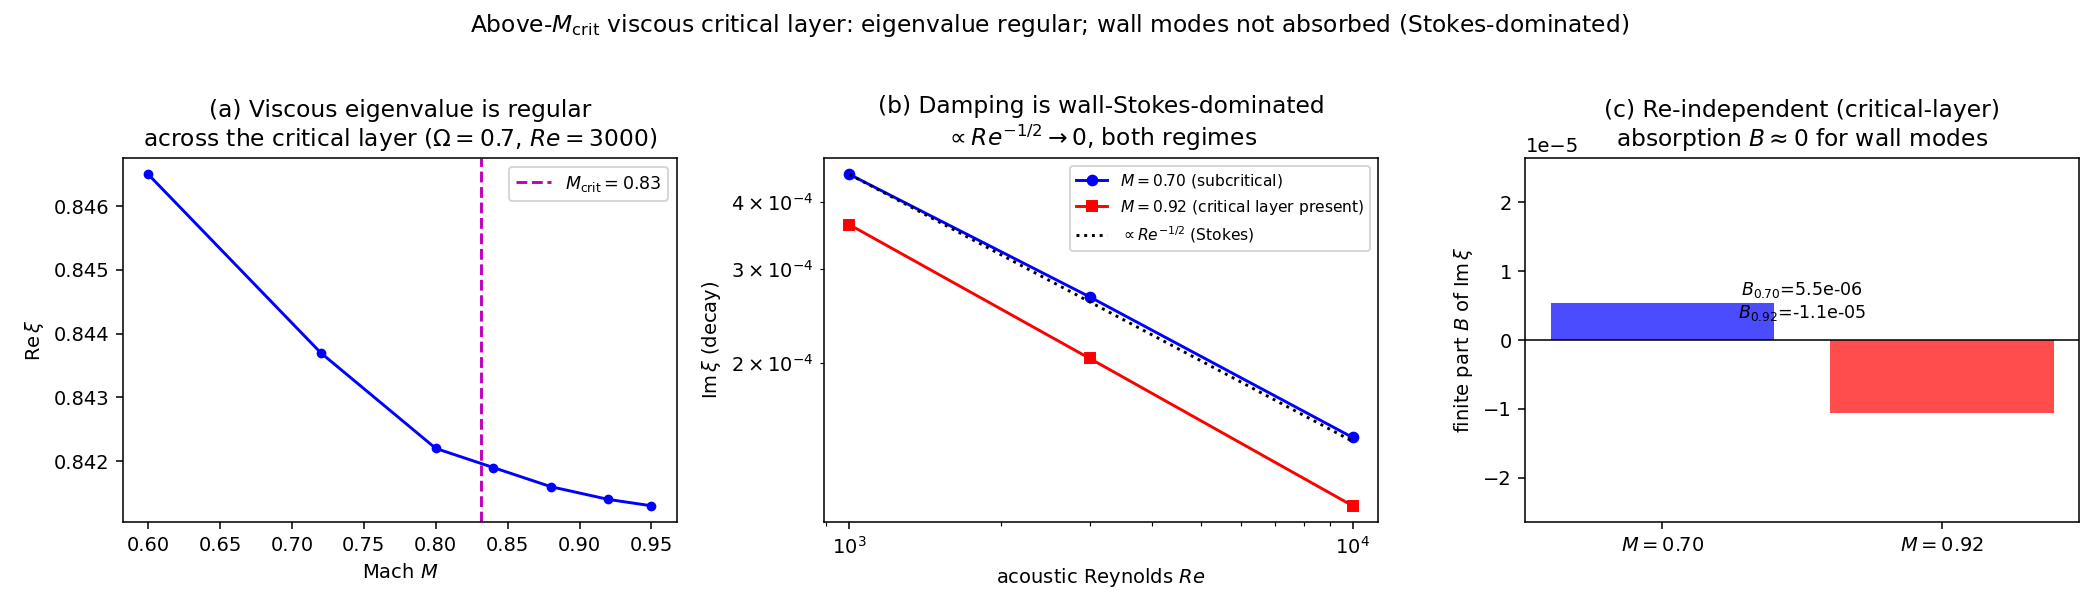
\includegraphics[width=0.98\textwidth]{fig8_viscous_global.png}
\caption{Viscous solution above $M_{\rm crit}$ ($\Om=0.7$). (a) The eigenvalue is regular through the
critical layer ($Re=3000$). (b) The decay rate $\operatorname{Im}\xi\propto Re^{-1/2}$ both below
($M{=}0.70$) and above ($M{=}0.92$) $M_{\rm crit}$ --- wall-Stokes-dominated, vanishing inviscidly.
(c) The $Re$-independent critical-layer absorption $B\approx0$: the discrete wall modes are not
absorbed by the interior critical layer.}
\label{fig:viscglobal}
\end{figure}

\section{Numerical validation}\label{sec:val}
The analytical results are confirmed by three mutually independent routes. (1) A Runge--Kutta
\emph{shooting} solver and an independent \emph{Chebyshev spectral collocation} eigensolver for
\eqref{eq:pb} agree to $\sim\!6\times10^{-9}$ on every branch for $M$ up to $0.2$. (2) Both reduce, at
$M=0$, to the symbolically verified closed-form quiescent relation \eqref{eq:disp}. (3) A
\emph{primitive-variable} (linearised-Euler, three-field $u',v',p'$) formulation, eliminated
symbolically, reproduces the Pridmore--Brown operator \eqref{eq:pb} exactly; this independent
derivation fixed the sign of the shear term. The closed-form $O(M)$ coefficient \eqref{eq:xi1} matches
the numerical $d\xi/dM$ to $0.1$--$0.5\%$ (Table~\ref{tab:xi1}); the symmetric branch of the
quiescent problem reproduces the Sarkar--Sonti single-plate result with $(a,\eps)\to(a/2,\eps/2)$ to
four decimals at every frequency.

\begin{table}[h]
\centering
\begin{tabular}{ccccc}
\toprule
$\Om$ & branch ($\xi_0$) & type & $\xi_1$ (closed) & $\xi_1$ (numerical)\\
\midrule
1.3 & 1.1165 & sym structural & $-0.1283$ & $-0.1290$\\
1.3 & 1.1837 & anti structural & $-0.1065$ & $-0.1068$\\
1.3 & 1.3267 & plane wave & $-0.7471$ & $-0.7468$\\
1.8 & 1.8069 & plane wave & $-1.1743$ & $-1.1750$\\
\bottomrule
\end{tabular}
\caption{Closed-form $O(M)$ correction \eqref{eq:xi1} vs.\ numerical $d\xi/dM$ ($l=3$, $\eps=0.25$).}
\label{tab:xi1}
\end{table}

\begin{figure}[h]
\centering
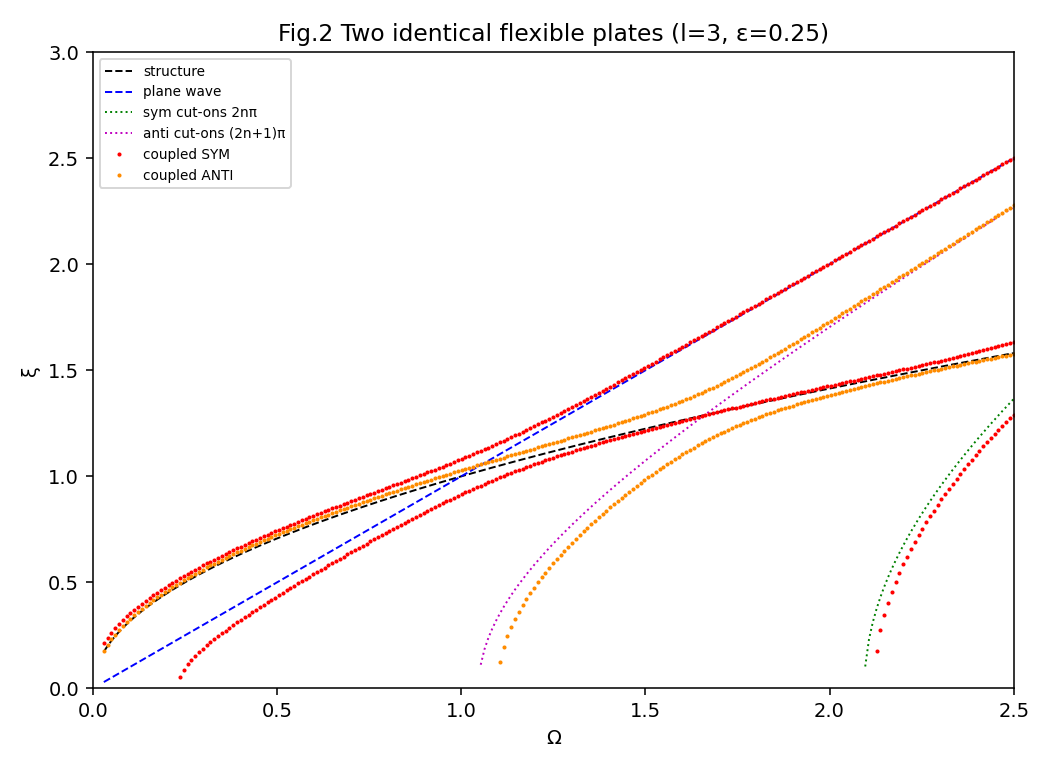
\includegraphics[width=0.9\textwidth]{fig2_two_identical.png}
\caption{Coupled symmetric and antisymmetric dispersion branches for two identical flexible plates
($l=3$, $\eps=0.25$), overlaid on the uncoupled parents. The symmetric family tracks the plane wave
and even cut-ons, the antisymmetric family the odd cut-ons; both perturb the common structural wave
and open gaps at every intersection.}
\label{fig:branches}
\end{figure}

\begin{figure}[h]
\centering
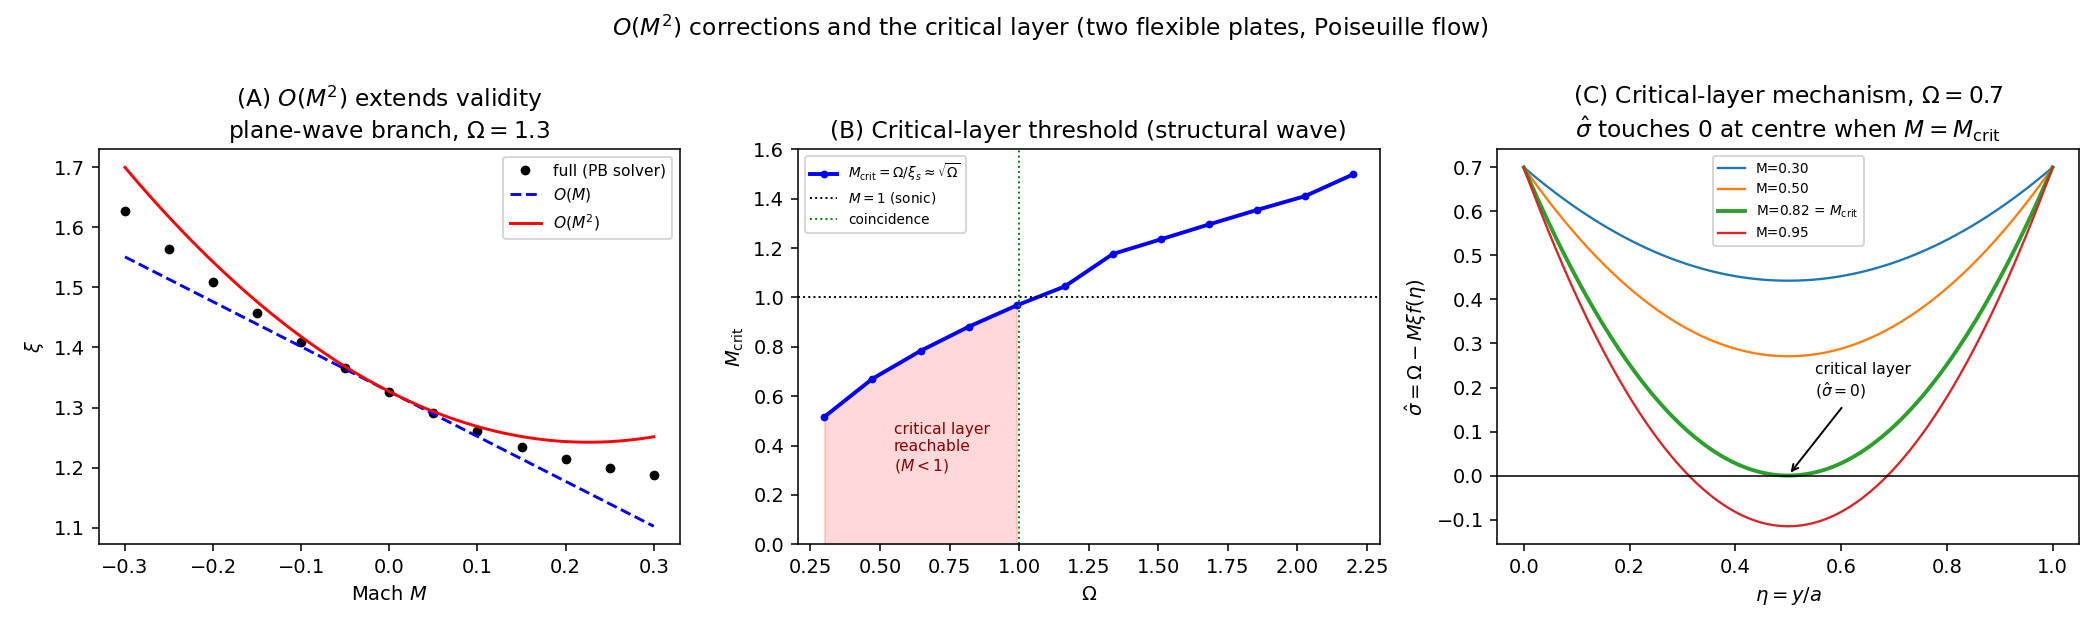
\includegraphics[width=0.98\textwidth]{fig6_om2_critical.png}
\caption{Mean-flow effects. (a) $O(M^2)$ extends the validity of the asymptotic wavenumber beyond
$O(M)$. (b) Critical-layer threshold $M_{\rm crit}=\Om/\xi_s\approx\sqrt{\Om}$ (reachable at subsonic
$M$ only below coincidence). (c) The Doppler-shifted frequency $\hat\sigma(\eta)$ touches zero at the
centreline when $M=M_{\rm crit}$.}
\label{fig:meanflow}
\end{figure}

\begin{figure}[h]
\centering
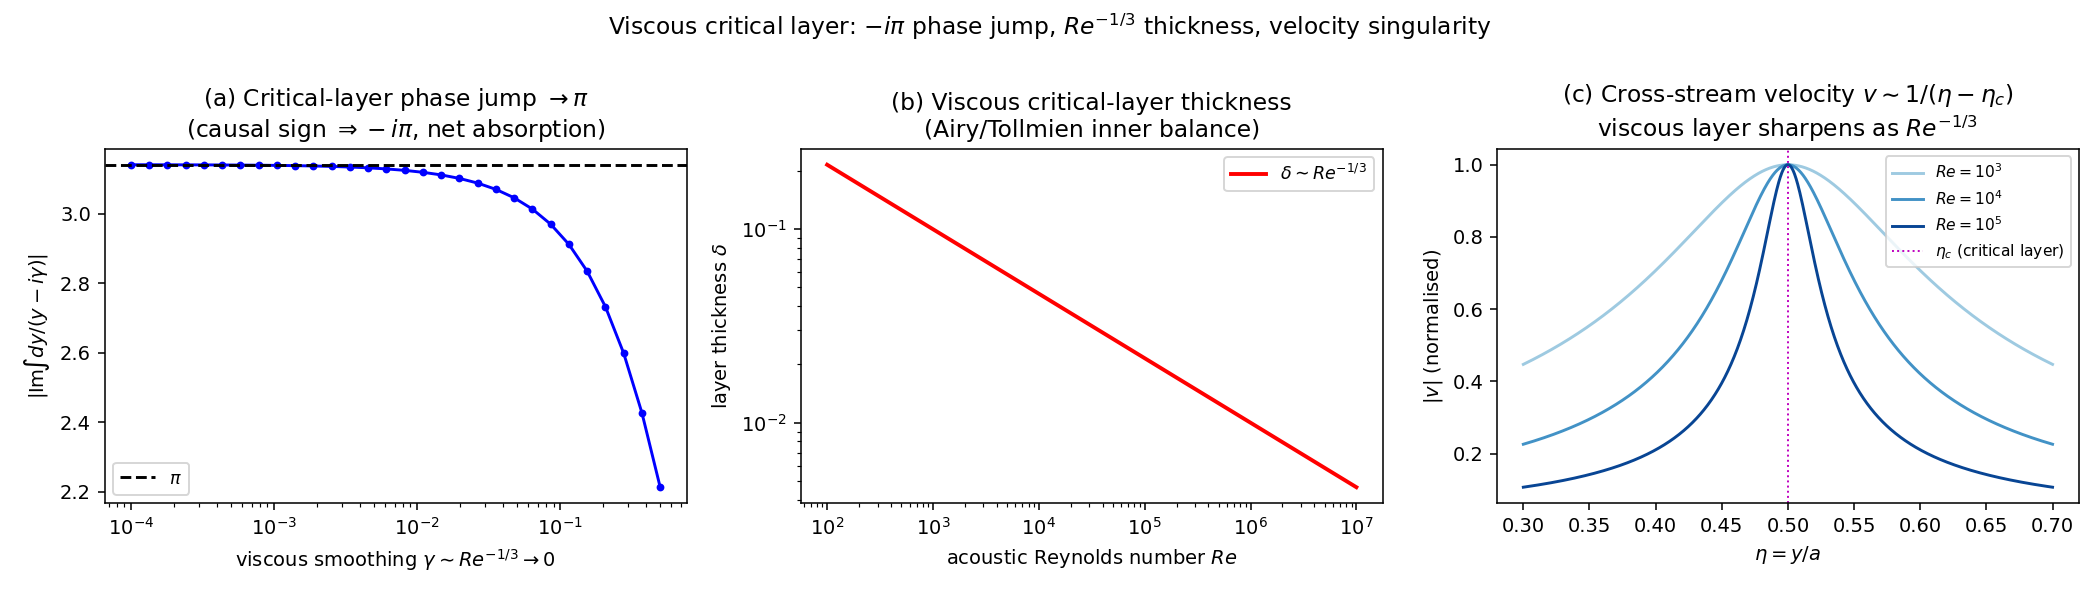
\includegraphics[width=0.98\textwidth]{fig7_viscous_cl.png}
\caption{Viscous critical layer. (a) The causal phase jump tends to $\pi$ in magnitude as the viscous
smoothing vanishes ($-\mathrm{i}\pi$, net absorption). (b) Inner-layer thickness $\delta\sim Re^{-1/3}$.
(c) The cross-stream velocity singularity $v\sim(\eta-\eta_c)^{-1}$, regularised over a layer that
sharpens as $Re^{-1/3}$.}
\label{fig:viscous}
\end{figure}

\section{Results and discussion}
The two-flexible-plate waveguide reduces correctly to all known limits and adds qualitatively new
behaviour. The cut-on spectrum is twice as dense as the single-plate spectrum, organised into
interleaved symmetric (even) and antisymmetric (odd) ladders; only the symmetric family inherits the
plane wave and the coincidence gap, while the antisymmetric structural wave traverses coincidence
regularly (Fig.~\ref{fig:branches}). For non-identical plates the symmetry decoupling is lost and the
two structural waves veer (avoided crossing), with minimum gap
$\Delta\xi=\eps/[2l\sqrt{\Om-1}\sin\tau_s]$ at $r_D=r_m=1$, scaling linearly in $\eps$. A structural
loss factor renders the wavenumbers complex, the structural branches attenuating most strongly and the
plane wave least.

The mean flow Doppler-shifts every branch at $O(M)$ and adds a direction-independent $O(M^2)$
correction in which shear is significant (Fig.~\ref{fig:meanflow}). The critical-layer threshold
cleanly separates a regular subsonic-flow regime (in which the present low-Mach asymptotics apply)
follows the classical $Re^{-1/3}$ inner-layer structure, with the important qualification that the
\emph{wall-driven discrete modes couple only weakly to the interior critical layer}: the viscous
linearised Navier--Stokes solution (Fig.~\ref{fig:viscglobal}) shows the eigenvalue remains regular
through and above $M_{\rm crit}$, with a decay rate that is wall-Stokes-dominated ($\propto Re^{-1/2}$)
and a vanishing $Re$-independent critical-layer absorption. The strong singular critical-layer
response is therefore confined to the cross-stream velocity field and the continuous spectrum, rather
than the discrete wavenumbers.

\section{Larger Mach numbers: full dispersion, validity and stability}
The closed-form corrections of \S4.1 are asymptotic in $M$; for larger Mach numbers the full
nonlinear-in-$M$ dispersion is obtained directly from \eqref{eq:pb}. Figure~\ref{fig:Mmap} maps every
coupled branch for $M=0,0.3,0.5$: increasing downstream flow shifts the entire diagram to lower $\xi$
(consistent with $\xi_1<0$), most strongly for the plane-wave-like branch and least for the
structural branches, while the cut-on ladder structure is preserved. We stress a physical-validity
limit: a strictly parabolic Poiseuille profile is a low-Mach idealisation, so the model is quantitative
for centreline Mach numbers up to the transonic range and is reported here as a model extension rather
than a compressible-mean-flow prediction.

The validity boundary of the asymptotics is branch-dependent (Fig.~\ref{fig:valid}a,b): for the
flow-sensitive plane-wave branch the $O(M)$ and $O(M^2)$ expansions exceed $5\%$ error by
$M\approx0.25$--$0.3$ (and the series, being asymptotic, ultimately diverges), whereas for a
flow-insensitive structural branch they remain accurate ($\lesssim3\%$) to much larger $M$. Thus the
closed-form corrections are quantitative at low $M$ and the full solver is required beyond
$M\sim0.3$ on the sensitive branches.

Finally, the convective stability of the coupled system was assessed by computing the complex
wavenumber with the viscous solver: the inviscid eigenvalues remain real and the viscous decay rate
satisfies $\operatorname{Im}\xi>0$ throughout the studied range (Fig.~\ref{fig:valid}c), i.e.\ the
mean flow does not destabilise the structural-acoustic wall modes (no flow-induced flutter) up to the
transonic limit of the model; the damping is wall-Stokes-dominated and vanishes inviscidly.

\begin{figure}[h]
\centering
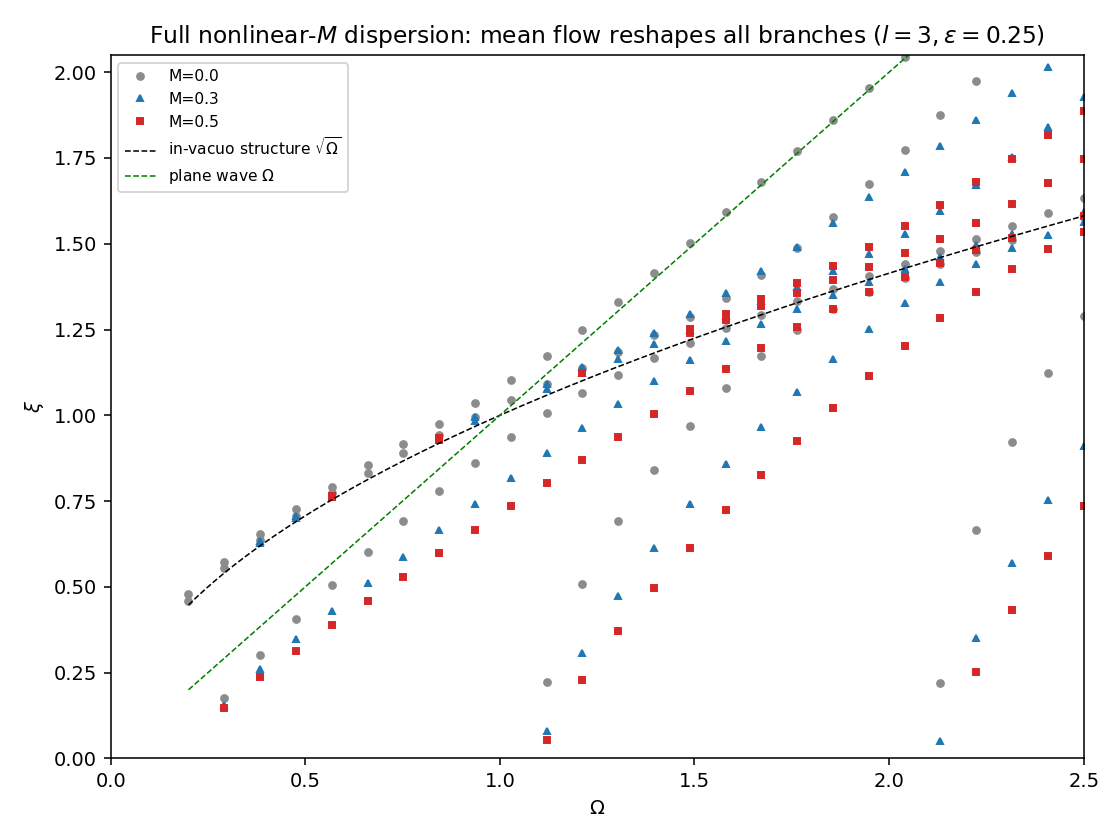
\includegraphics[width=0.72\textwidth]{fig9_Mmap.png}
\caption{Full nonlinear-in-$M$ dispersion ($l=3$, $\eps=0.25$): mean flow shifts every coupled branch
to lower $\xi$ with increasing downstream Mach number, most strongly near the plane wave.}
\label{fig:Mmap}
\end{figure}

\begin{figure}[h]
\centering
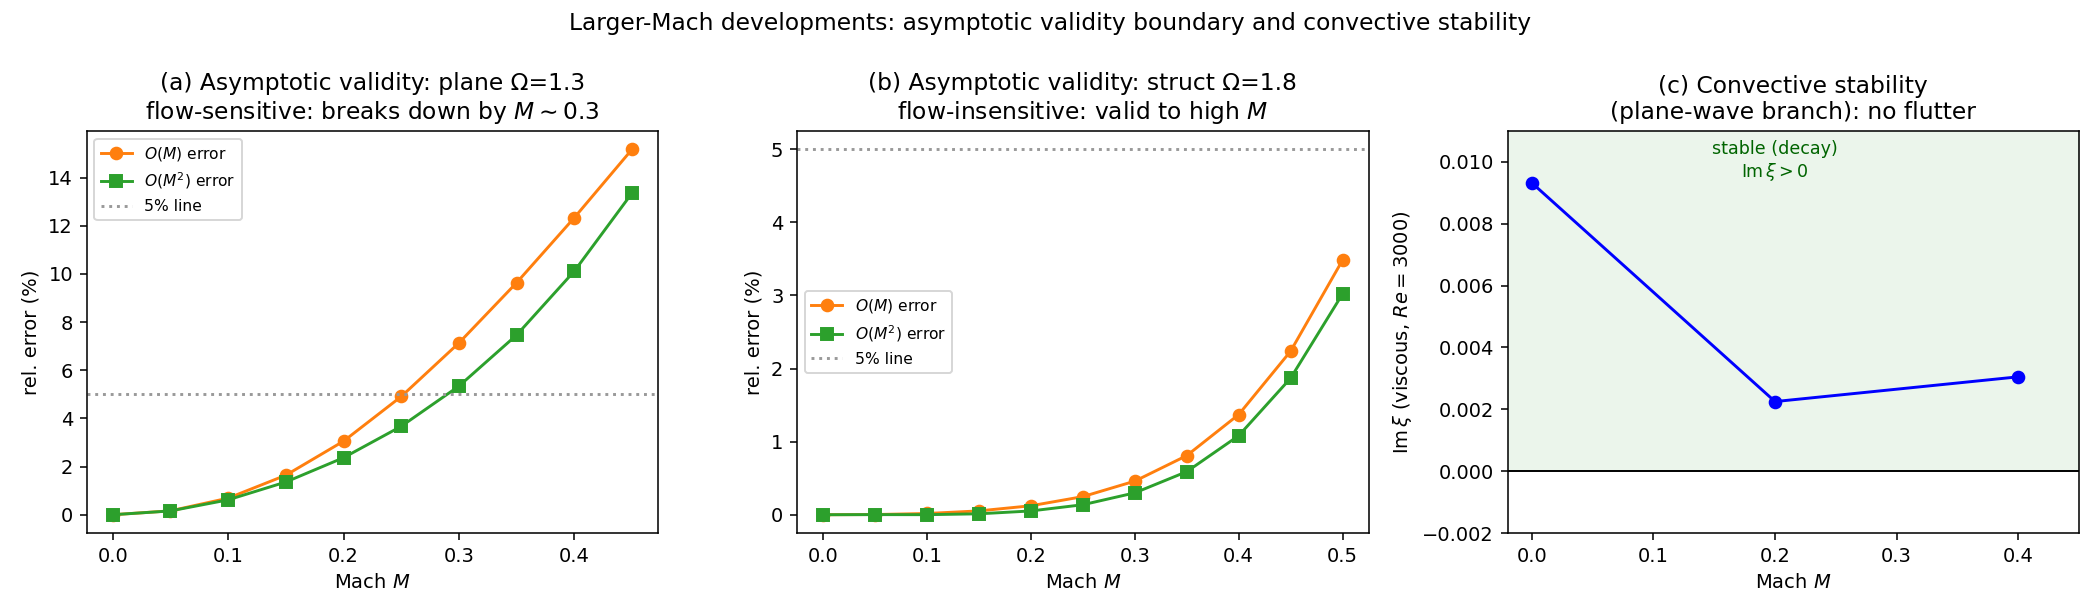
\includegraphics[width=0.99\textwidth]{fig10_validity_stability.png}
\caption{(a,b) Branch-dependent validity of the $O(M)$/$O(M^2)$ asymptotics: the flow-sensitive
plane-wave branch breaks down by $M\sim0.3$, while a flow-insensitive structural branch stays accurate
to larger $M$. (c) Convective stability: the viscous decay rate $\operatorname{Im}\xi>0$ (no flutter).}
\label{fig:valid}
\end{figure}

\section{Conclusions}
Closed-form asymptotic expressions have been derived and numerically validated for the coupled
wavenumbers of a fluid column bounded by two flexible plates, generalising Sarkar \& Sonti and Fahy to
both symmetry families and to non-identical plates, and extended to a low-Mach Poiseuille mean flow via
the Pridmore--Brown equation with a closed-form $O(M)$ correction, an $O(M^2)$ convection/shear split,
and a critical-layer analysis. A viscous linearised Navier--Stokes solution shows the eigenvalue is
regular above $M_{\rm crit}$ and that the discrete wall modes are not absorbed by the critical layer
(their decay is wall-Stokes-dominated, $\propto Re^{-1/2}$, vanishing inviscidly). Three independent
numerical methods confirm the results. The framework is simple to implement symbolically and
physically transparent, and provides design-oriented expressions for compliant ducts and flow-bearing
elastic waveguides. The nonlinear (finite-amplitude) critical layer and the continuous-spectrum
contribution remain for future work.


\appendix
\section{Plate-admittance boundary conditions}\label{app:bc}
We derive the wall conditions used with the Pridmore--Brown equation~\eqref{eq:pb}, in both the
inviscid and viscous formulations, and show their consistency. Fields vary as
$e^{\mathrm{i}(\omega t-k_xx)}$ so that $\mathrm{D}/\mathrm{D}t=\partial_t+U\partial_x\to
\mathrm{i}(\omega-k_xU)=\mathrm{i}\sigma$. \emph{Crucially, the Poiseuille profile is no-slip,
$U(0)=U(a)=0$, so at each wall $\sigma\to\omega$ and the material derivative reduces to $\partial_t$};
the convective (Ingard--Myers) slip correction therefore vanishes at the walls.

\paragraph{Kinematic and plate-dynamic conditions.} Continuity of normal velocity gives
$v=\mathrm{D}w_j/\mathrm{D}t$, which at the walls (where $U=0$) is $v=\mathrm{i}\omega w_j$. The thin
plates satisfy $G_jw_j=\mp p$ ($-$ at $y=0$, fluid above plate~1; $+$ at $y=a$, fluid below plate~2),
with $G_j=D_jk_x^4-m_j\omega^2$. Eliminating $w_j$,
\begin{equation}
v(0)=-\frac{\mathrm{i}\omega}{G_1}\,p(0),\qquad v(a)=+\frac{\mathrm{i}\omega}{G_2}\,p(a).
\label{eq:adm}
\end{equation}

\paragraph{Inviscid form (used in \eqref{eq:pb}).} The inviscid $y$-momentum equation
$\rho\,\mathrm{D}v/\mathrm{D}t=-\partial_yp$ gives $v=\mathrm{i}\,p_y/(\sigma\rho)$, so at $y=0$
($\sigma=\omega$) $v(0)=\mathrm{i}\,p_y(0)/(\omega\rho)$. Equating to \eqref{eq:adm} yields
$p_y(0)=-\omega^2\rho\,p(0)/G_1$. Non-dimensionalising ($\hat p=p/\rho c^2$, $\eta=y/a$,
$G_1=m_1\omega^2S_1$, $\varepsilon=\rho a/m_1$),
\begin{equation}
\hat p_\eta(0)+\frac{\varepsilon}{S_1}\hat p(0)=0,\qquad
\hat p_\eta(1)-\frac{\varepsilon}{S_2}\hat p(1)=0,
\label{eq:robinp}
\end{equation}
which are the plate-admittance (Robin) conditions imposed on the Pridmore--Brown pressure.

\paragraph{Viscous form (linearised Navier--Stokes, \S4.3).} When viscosity is retained the velocity
is no longer slaved to $p_y$; instead the pressure follows from the (inviscid-energy) continuity
relation $\mathrm{i}\sigma\,p+\rho c^2(-\mathrm{i}k_xu+\partial_yv)=0$, i.e.\ in non-dimensional form
$\hat p=\xi\hat u/\hat\sigma+\mathrm{i}\hat v_\eta/(l\hat\sigma)$. Imposing no-slip $\hat u=0$ at the
wall (and $\hat\sigma=\Omega$ there) gives $\hat p(0)=\mathrm{i}\hat v_\eta(0)/(l\Omega)$. The
non-dimensional admittance \eqref{eq:adm}, $\hat v(0)=-\mathrm{i}\varepsilon\hat p(0)/(l\Omega S_1)$,
then becomes a Robin condition on the normal velocity,
\begin{equation}
\hat v(0)-\beta_1\hat v_\eta(0)=0,\qquad \hat v(1)+\beta_2\hat v_\eta(1)=0,\qquad
\beta_j=\frac{\varepsilon}{l^2\Omega^2S_j}.
\label{eq:robinv}
\end{equation}
As $Re\to\infty$ the viscous $y$-momentum balance reduces to the inviscid one and \eqref{eq:robinv}
reduces to \eqref{eq:robinp}; both reductions, and the coefficients $\beta_j$, were verified
symbolically. No-slip ($\hat u=0$) and \eqref{eq:robinv} furnish the four boundary conditions required
by the fourth-order viscous system.
\begin{thebibliography}{9}
\bibitem{sarkarsonti} A.\ Sarkar, V.R.\ Sonti, An asymptotic analysis for the coupled dispersion
characteristics of a structural acoustic waveguide, \emph{J.\ Sound Vib.}\ \textbf{306} (2007) 657--674.
\bibitem{fahy} F.\ Fahy, \emph{Sound and Structural Vibration: Radiation, Transmission and Response},
Academic Press, 1989, pp.\ 259--268, 136--140.
\bibitem{kunte2011} A.\ Sarkar, M.V.\ Kunte, V.R.\ Sonti, Unified dispersion characteristics of
structural acoustic waveguides, \emph{Comput.\ Model.\ Eng.\ Sci.}\ \textbf{81} (3\&4) (2011) 249--268.
\bibitem{prakash2016} V.\ Prakash, V.R.\ Sonti, A systematic asymptotic approach to determine the
dispersion characteristics of structural-acoustic waveguides with arbitrary fluid loading,
\emph{J.\ Sound Vib.}\ \textbf{373} (2016) 164--179.
\bibitem{morseingard} P.M.\ Morse, K.U.\ Ingard, \emph{Theoretical Acoustics}, McGraw--Hill, 1968,
pp.\ 624--634.
\bibitem{crighton} D.G.\ Crighton, The 1988 Rayleigh Medal Lecture: fluid loading---the interaction
between sound and vibration, \emph{J.\ Sound Vib.}\ \textbf{133} (1) (1989) 1--27.
\bibitem{pridmorebrown} D.C.\ Pridmore-Brown, Sound propagation in a fluid flowing through an
attenuating duct, \emph{J.\ Fluid Mech.}\ \textbf{4} (1958) 393--406.
\bibitem{brambley} E.J.\ Brambley, A well-posed boundary condition for acoustic liners in straight
ducts with flow, \emph{AIAA J.}\ \textbf{49} (6) (2011) 1272--1282.
\bibitem{brambleydarau} E.J.\ Brambley, M.\ Darau, S.W.\ Rienstra, The critical layer in linear-shear
boundary layers over acoustic linings, \emph{J.\ Fluid Mech.}\ \textbf{710} (2012) 545--568.
\bibitem{maslowe} S.A.\ Maslowe, Critical layers in shear flows, \emph{Annu.\ Rev.\ Fluid Mech.}\
\textbf{18} (1986) 405--432.
\bibitem{morab} S.R.\ Morab, A.\ Sharma, J.S.\ Murallidharan, Low Mach number approximated linearized
perturbed Euler equations-based unified computational flow-induced acoustic model for 2D
planar/axisymmetric complex geometry, \emph{J.\ Comput.\ Phys.}\ \textbf{514} (2024) 113242.
\end{thebibliography}

\end{document}
